\documentclass[conference]{IEEEtran}
\IEEEoverridecommandlockouts

\usepackage[T1]{fontenc}
\usepackage{cite}
\usepackage{amsmath,amssymb}
\usepackage{graphicx}
\usepackage{booktabs}
\usepackage{array}
\usepackage{xcolor}
\usepackage{listings}
\usepackage{tikz}
\usetikzlibrary{arrows.meta,positioning,fit,backgrounds,shapes.geometric,calc}
\usepackage[hidelinks]{hyperref}
\usepackage{url}

% Placeholder marker for facts the author must confirm before submission.
\newcommand{\tbd}[1]{\textcolor{red}{[#1]}}

\lstset{
  basicstyle=\ttfamily\scriptsize,
  breaklines=true,
  breakatwhitespace=false,
  columns=fullflexible,
  keepspaces=true,
  frame=single,
  framerule=0.3pt,
  rulecolor=\color{black!40},
  backgroundcolor=\color{black!3},
  xleftmargin=2pt,
  xrightmargin=2pt,
  aboveskip=4pt,
  belowskip=4pt
}

\begin{document}

\title{Drop-In Hybrid Post-Quantum Key Exchange for TLS~1.3 at Zero Trust Boundaries: Architecture, Functional Validation, and an Open Evaluation Agenda}

\author{\IEEEauthorblockN{Raj Sahasranamam\thanks{ORCID: 0009-0001-4855-6601}}
\IEEEauthorblockA{Nila Professional Services\\
Monroe Township, New Jersey, USA\\
kumar@nilaproservices.com}}

\maketitle

\begin{abstract}
Adversaries can record encrypted traffic today and decrypt it once a cryptographically relevant quantum computer exists. This ``harvest now, decrypt later'' threat makes key establishment the most urgent target for post-quantum migration, ahead of authentication. This paper presents a reference architecture for upgrading Transport Layer Security (TLS) 1.3 at Zero Trust boundaries by changing only the key exchange: elliptic-curve Diffie-Hellman is replaced by the hybrid group X25519MLKEM768, which combines X25519 with the NIST-standardized ML-KEM-768 and is now specified in RFC~10024. Applications, X.509 certificates, and symmetric cipher suites remain unchanged. We map the architecture to five boundary classes common in defense and commercial environments, document a reproducible procedure for Windows and Linux using OpenSSL~3.5, and report functional validation showing that the hybrid group is negotiated with the cipher suite and certificate untouched. We then describe two vendor-neutral architectural extensions, quantum random number generator entropy integration and Ising/QUBO-based operational optimization, which are proposed and not evaluated here. Finally, we define an open evaluation agenda with a test matrix and testable hypotheses, and release the procedure as an open artifact to invite community measurement.
\end{abstract}

\begin{IEEEkeywords}
post-quantum cryptography, ML-KEM, hybrid key exchange, TLS 1.3, Zero Trust, crypto-agility, harvest now decrypt later
\end{IEEEkeywords}

\section{Introduction}

Shor's algorithm~\cite{shor1994} breaks the integer factorization and discrete logarithm problems that underpin RSA and elliptic-curve cryptography (ECC). No quantum computer capable of doing so at cryptographic scale exists today, but the timing question is asymmetric. Mosca~\cite{mosca2018} frames it as an inequality: if the time data must remain confidential ($x$) plus the time needed to migrate ($y$) exceeds the time until a cryptographically relevant quantum computer (CRQC) exists ($z$), then data is already at risk. Traffic captured today under classical key exchange can be stored and decrypted later. Authentication, by contrast, only needs to resist an adversary at the moment a handshake occurs.

Policy has followed this logic. NIST published the Module-Lattice-Based Key-Encapsulation Mechanism (ML-KEM) as FIPS~203 in August 2024~\cite{fips203}. NIST IR~8547, still an initial public draft, proposes deprecating quantum-vulnerable public-key algorithms after 2030 and disallowing them after 2035~\cite{nistir8547}. For U.S. National Security Systems, the NSA's CNSA~2.0 calls for web browsers, servers, and cloud services to support and prefer quantum-resistant algorithms by 2025 and to use them exclusively by 2033, with ML-KEM-1024 as the key-establishment algorithm~\cite{cnsa2}. NSM-10~\cite{nsm10} and OMB M-23-02~\cite{omb2302} direct federal agencies to inventory and migrate vulnerable systems. In parallel, the IETF has standardized hybrid key agreement for TLS~1.3 in RFC~10024~\cite{rfc10024}, and OpenSSL~3.5 ships ML-KEM with X25519MLKEM768 among its default key shares~\cite{openssl35}.

The standards now exist, yet practitioners responsible for specific boundaries (a portal, a service mesh hop, a cloud access point) still need a concrete answer to a narrower question: \emph{what is the smallest change that removes harvest-now-decrypt-later exposure on this link, and how do I prove it happened?} This paper answers that question for TLS~1.3.

\subsection{Contributions}
\begin{enumerate}
  \item A reference architecture for drop-in hybrid key exchange that changes only the TLS~1.3 key share, mapped to five boundary classes found in Department of Defense (DoD) and commercial Zero Trust deployments (Section~\ref{sec:arch}).
  \item A reproducible cross-platform procedure for OpenSSL~3.5 and functional validation evidence that X25519MLKEM768 is negotiated with the certificate and cipher suite unchanged, including practitioner pitfalls (Section~\ref{sec:validation}).
  \item Two vendor-neutral architectural extensions, quantum entropy integration and Ising/QUBO-based optimization, with explicit evaluation criteria, presented as proposals rather than results (Section~\ref{sec:extensions}).
  \item An open evaluation agenda: a test matrix, metrics, and falsifiable hypotheses, released with the procedure so that other researchers can contribute measurements (Section~\ref{sec:agenda}).
\end{enumerate}

\subsection{Scope}
This is a practitioner architecture and functional-validation paper. It does not report performance measurements. All validation was performed on a single Windows host over the loopback interface. We state this plainly because the distinction between ``the mechanism works'' and ``the mechanism performs acceptably at scale'' is exactly what the open evaluation agenda is designed to close.

\section{Background and Related Work}

\subsection{TLS 1.3 Key Establishment}
In TLS~1.3~\cite{rfc8446}, the client sends one or more \texttt{key\_share} entries in its ClientHello, each tagged with a named group. The server selects one group and replies with its own share in the ServerHello. The resulting shared secret feeds the HKDF-based key schedule, which derives all traffic keys. Because group negotiation is already a first-class protocol mechanism, introducing a new group requires no change to the record layer, cipher suites, or certificate handling.

\subsection{ML-KEM and Hybrid Groups}
ML-KEM is a key-encapsulation mechanism (KEM): the client sends an encapsulation key, and the server returns a ciphertext that encapsulates a shared secret. RFC~10024~\cite{rfc10024} defines three hybrid groups that pair ML-KEM with a classical elliptic-curve exchange. Table~\ref{tab:groups} summarizes their wire sizes as specified in the RFC. These are specification values, not measurements.

\begin{table}[t]
\centering
\caption{Key Share Sizes for Classical and Hybrid TLS~1.3 Groups (Specification Values From RFC~10024 and RFC~8446)}
\label{tab:groups}
\footnotesize
\setlength{\tabcolsep}{3.5pt}
\begin{tabular}{@{}lrrrc@{}}
\toprule
Group & Code & Client (B) & Server (B) & Order \\
\midrule
X25519 & 0x001D & 32 & 32 & EC \\
secp256r1 & 0x0017 & 65 & 65 & EC \\
X25519MLKEM768 & 0x11EC & 1216 & 1120 & PQ, EC \\
SecP256r1MLKEM768 & 0x11EB & 1249 & 1153 & EC, PQ \\
SecP384r1MLKEM1024 & 0x11ED & 1665 & 1665 & EC, PQ \\
\bottomrule
\multicolumn{5}{@{}p{0.95\columnwidth}@{}}{\scriptsize Order: concatenation order of components in the key share. PQ: ML-KEM; EC: elliptic-curve.} \\
\end{tabular}
\end{table}

The hybrid shared secret is the concatenation of both component secrets, which then enters the standard TLS~1.3 key schedule. Bindel et al.~\cite{bindel2019} analyze such combiners and show that the derived key remains secure if at least one component remains secure. This property is the core argument for hybrid deployment during the transition: an unexpected weakness in the young ML-KEM implementation ecosystem is backstopped by X25519, and a future CRQC that breaks X25519 is stopped by ML-KEM.

\subsection{Prior Measurement Work}
Paquin, Stebila, and Tamvada~\cite{paquin2020} benchmarked post-quantum key exchange and signatures in TLS under emulated network conditions and found that as packet loss rises, schemes with larger handshake messages are disproportionately affected, an effect that loopback testing cannot reveal. Sikeridis, Kampanakis, and Devetsikiotis~\cite{sikeridis2020} studied post-quantum authentication in TLS~1.3 and showed that the choice of signature scheme and the resulting certificate-chain size strongly affect handshake cost when authentication is upgraded. Both lines of work motivate our separation of concerns: key exchange first, authentication later, and measurement as a distinct, community-scale effort.

\subsection{Zero Trust Boundaries}
NIST SP~800-207~\cite{sp800207} and the DoD Zero Trust Strategy~\cite{dodzt} treat every connection as untrusted until verified and push encryption to every hop. A consequence is that the number of TLS-terminating boundaries grows sharply: user-to-portal sessions, service-to-service mutual TLS, gateway crossings, and API brokers. Each is a separate harvest-now-decrypt-later exposure, which makes a repeatable, per-boundary upgrade pattern more valuable than a one-time network-wide change.

\section{Threat Model}
\label{sec:threat}

\textbf{Adversary.} A passive network adversary records TLS traffic today and later obtains a CRQC capable of running Shor's algorithm against the classical key exchange.

\textbf{Asset.} The confidentiality of application data carried over TLS~1.3 sessions whose sensitivity lifetime ($x$ in Mosca's terms) extends beyond the expected arrival of a CRQC.

\textbf{In scope.} Recovery of session keys from recorded handshakes. A hybrid key exchange defeats this if ML-KEM-768 resists quantum attack.

\textbf{Out of scope.} (i) Active, real-time man-in-the-middle attacks using a CRQC to forge classical signatures; these require post-quantum authentication (for example ML-DSA certificates), which we defer. (ii) Implementation side channels. (iii) Endpoint compromise. (iv) Downgrade attacks by an active classical adversary, which TLS~1.3's transcript-bound handshake already resists, though deployment configuration (Section~\ref{sec:limits}) matters.

The certificate in our validation uses RSA-2048. This is deliberate: it isolates the variable under test and reflects the realistic first migration step, in which existing public key infrastructure is left in place.

\section{Reference Architecture}
\label{sec:arch}

The design principle is minimal change: alter only the named group offered and accepted in the TLS~1.3 handshake. With OpenSSL~3.5 this change is largely a library upgrade, because X25519MLKEM768 and X25519 are the default key shares~\cite{openssl35}, so two 3.5 peers typically negotiate the hybrid group without any configuration. Explicit group configuration then serves a different purpose: it \emph{enforces} the hybrid group, preventing silent classical fallback, and makes the security property auditable. Fig.~\ref{fig:arch} shows the reference topology. A client endpoint (labelled \emph{Sensor} to reflect operational-technology and telemetry use cases) connects to a TLS-terminating \emph{Gateway}. An \emph{Observer} captures the handshake for evidence. Two optional extension points, drawn dashed, are discussed in Section~\ref{sec:extensions}.

\begin{figure}[t]
\centering
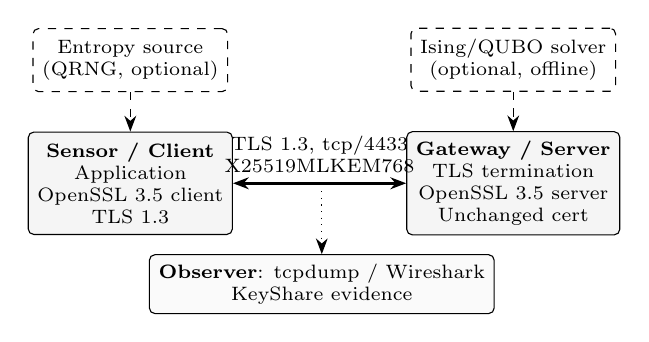
\begin{tikzpicture}[
  node distance=6mm and 10mm,
  box/.style={draw, rounded corners=2pt, align=center, font=\scriptsize, minimum width=24mm, minimum height=13mm, fill=black!4},
  ext/.style={draw, dashed, rounded corners=2pt, align=center, font=\scriptsize, minimum width=24mm, minimum height=8mm},
  obs/.style={draw, rounded corners=2pt, align=center, font=\scriptsize, minimum width=30mm, minimum height=7mm, fill=black!2},
  >={Stealth[length=2mm]}
]
\node[box] (s) {\textbf{Sensor / Client}\\Application\\OpenSSL 3.5 client\\TLS 1.3};
\node[box, right=22mm of s] (g) {\textbf{Gateway / Server}\\TLS termination\\OpenSSL 3.5 server\\Unchanged cert};
\draw[<->, very thick] (s.east) -- node[above, font=\scriptsize, align=center]{TLS 1.3, tcp/4433\\X25519MLKEM768} (g.west);
\node[obs, below=9mm of $(s)!0.5!(g)$] (o) {\textbf{Observer}: tcpdump / Wireshark\\KeyShare evidence};
\draw[->, dotted] ($(s)!0.5!(g)$) ++(0,-1mm) -- (o.north);
\node[ext, above=5mm of s] (q1) {Entropy source\\(QRNG, optional)};
\node[ext, above=5mm of g] (q2) {Ising/QUBO solver\\(optional, offline)};
\draw[->, dashed] (q1) -- (s);
\draw[->, dashed] (q2) -- (g);
\end{tikzpicture}
\caption{Reference topology. Only the TLS~1.3 named group changes. Dashed elements are proposed extensions (Section~\ref{sec:extensions}) and were not part of the validation.}
\label{fig:arch}
\end{figure}

\subsection{Boundary Mapping}
Table~\ref{tab:mapping} maps the lab link to five boundary classes. In each case the change is identical: the group configuration on the TLS terminator and its peer. This is what makes the pattern repeatable.

\begin{table}[t]
\centering
\caption{Mapping of the Reference Link to Operational Boundary Classes}
\label{tab:mapping}
\footnotesize
\begin{tabular}{@{}>{\raggedright\arraybackslash}p{0.33\columnwidth}>{\raggedright\arraybackslash}p{0.27\columnwidth}>{\raggedright\arraybackslash}p{0.30\columnwidth}@{}}
\toprule
Boundary class & Lab analogue & Where the group is set \\
\midrule
User to web application (HTTPS, CAC/PIV) & Client to gateway handshake & Portal load balancer or reverse proxy \\
Service to service (mTLS in a mesh) & One sensor to gateway hop & Mesh sidecar or proxy configuration \\
Enclave to cloud (cloud access point) & VM to VM link across a boundary & Boundary gateway or proxy pair \\
Secure file and records portals & Same HTTPS channel & Front-end TLS terminator \\
API gateways across enclaves & Gateway as API terminator & API gateway listener \\
\bottomrule
\end{tabular}
\end{table}

\subsection{Why Hybrid, Not Pure ML-KEM}
A pure ML-KEM group (\texttt{MLKEM768}) is also available in OpenSSL~3.5 and is useful in controlled labs. For production transition we recommend hybrid for three reasons: (i) the combiner property~\cite{bindel2019} protects against implementation or cryptanalytic surprises in either component; (ii) hybrid groups are the deployed and IETF-recommended path, which maximizes interoperability with current browsers, libraries, and middleboxes; and (iii) compliance regimes that still require a FIPS-validated classical component can be satisfied during the transition, with the ordering details in Table~\ref{tab:groups} determining which component's implementation must carry validation~\cite{rfc10024}.

\section{Implementation and Functional Validation}
\label{sec:validation}

\subsection{Environment}
Validation was performed on a single Windows~11 Pro host using a prebuilt 64-bit OpenSSL distribution from the 3.5 release series or later. The exact patch release was not recorded; the series is established by the KEM listing in Section~\ref{sec:evidence}, since native ML-KEM and the hybrid TLS groups first shipped in OpenSSL~3.5~\cite{openssl35}. Server and client ran in separate PowerShell sessions and communicated over \texttt{127.0.0.1:4433}. A short-lived RSA-2048 self-signed certificate with \texttt{CN=demo.local} was generated for the server. OpenSSL ran with its default configuration file and no provider flags, so only the built-in default provider was active. Randomness therefore came from OpenSSL's default deterministic random bit generator (DRBG), which on Windows is seeded from the operating system's Cryptography API: Next Generation (CNG) entropy source. The DRBG itself is OpenSSL's, not the operating system's; the distinction matters for FIPS claims (Section~\ref{sec:fips}).

\subsection{Procedure}
The procedure has four steps. First, confirm that the build exposes ML-KEM and the hybrid groups. Second, generate a lab certificate and open the port. Third, start the server restricted to the hybrid group. Fourth, connect with a client restricted to the same group.

\begin{lstlisting}
# 1. Confirm KEM support
openssl list -kem-algorithms
# 2. Lab certificate
openssl req -x509 -newkey rsa:2048 -nodes \
  -keyout server.key -out server.crt -days 7 \
  -subj "/CN=demo.local"
# 3. Server, hybrid group only
openssl s_server -accept 4433 -tls1_3 \
  -cert server.crt -key server.key \
  -groups X25519MLKEM768 -www
# 4. Client, hybrid group only
openssl s_client -connect 127.0.0.1:4433 -tls1_3 \
  -groups X25519MLKEM768 -brief -ign_eof
\end{lstlisting}

On Windows the commands are invoked through the full path to \texttt{openssl.exe}. On Linux they run unchanged; the Linux procedure is included in the artifact but was not executed in this study. Restricting both peers to a single group is intentional: it converts a silent fallback into a hard failure, so a successful connection is itself proof of the hybrid negotiation.

\subsection{Evidence}\label{sec:evidence}
The KEM listing (step 1) reported ML-KEM-512, ML-KEM-768, and ML-KEM-1024 under their FIPS~203 object identifiers (2.16.840.1.101.3.4.4.1 through .3), together with the hybrid groups X25519MLKEM768, X448MLKEM1024, SecP256r1MLKEM768, and SecP384r1MLKEM1024, all from the default provider. Fig.~\ref{fig:evidence} shows the server and client sessions. The client reported:

\begin{lstlisting}
CONNECTION ESTABLISHED
Protocol version: TLSv1.3
Ciphersuite: TLS_AES_256_GCM_SHA384
Peer certificate: CN=demo.local
Signature type: rsa_pss_rsae_sha256
Negotiated TLS1.3 group: X25519MLKEM768
\end{lstlisting}

\begin{figure*}[t]
\centering
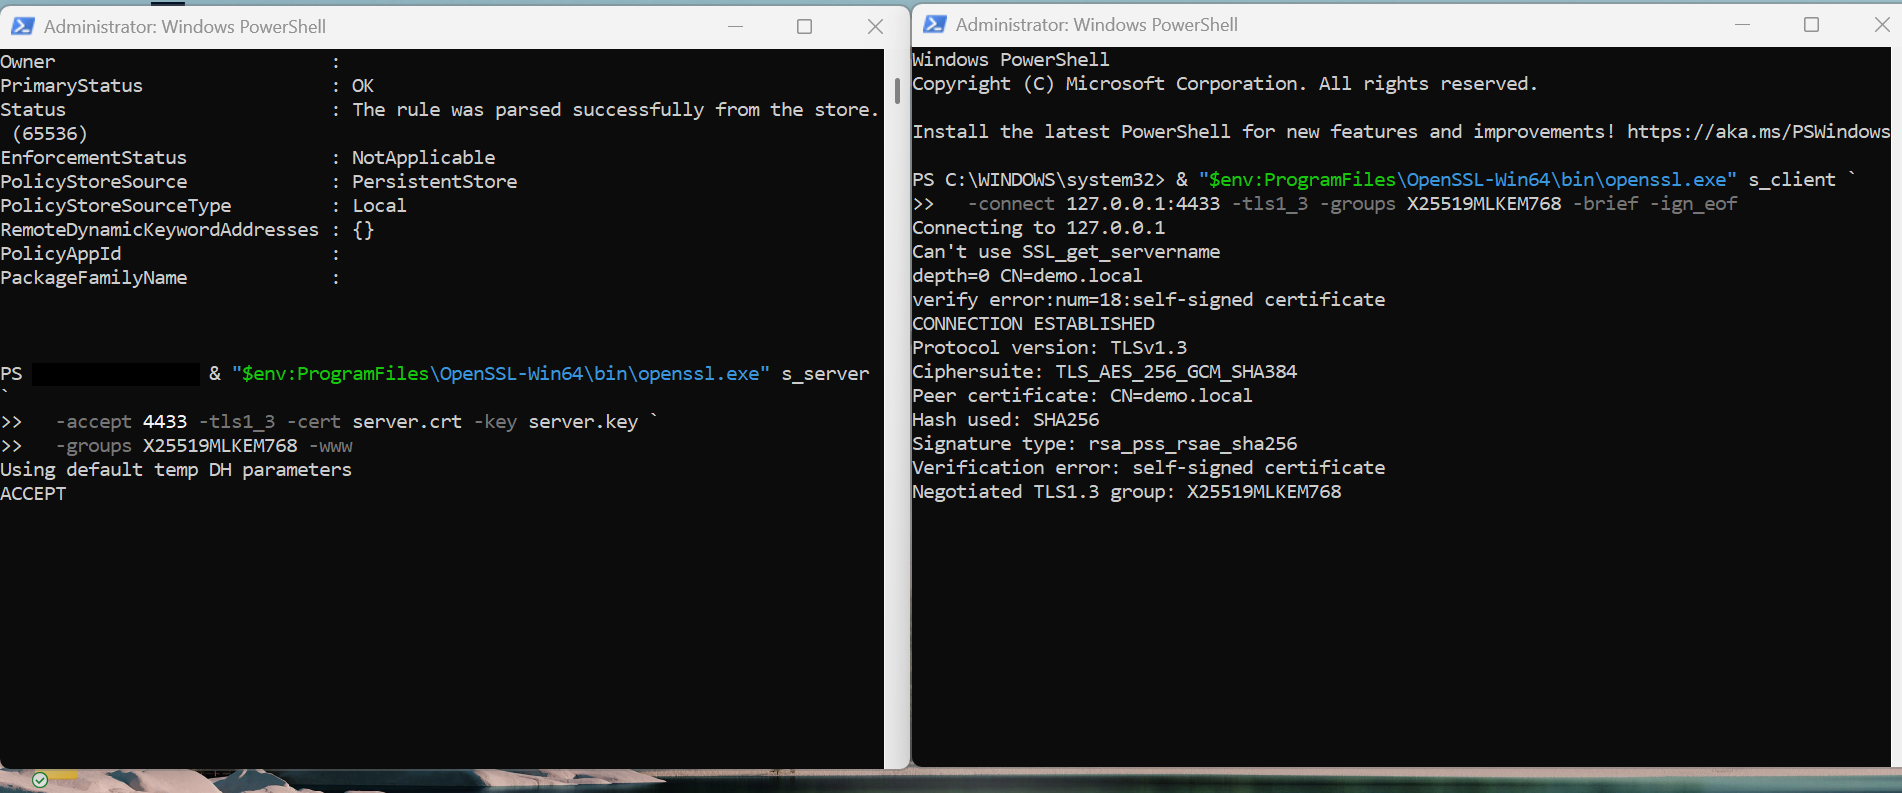
\includegraphics[width=0.92\textwidth]{figs/handshake_evidence.png}
\caption{Functional validation on Windows. Left: server restricted to X25519MLKEM768, in ACCEPT state. Right: client output showing TLS~1.3, the unchanged AES-256-GCM cipher suite, the RSA-PSS certificate signature, and the negotiated hybrid group. A local user path has been redacted.}
\label{fig:evidence}
\end{figure*}

The client also reported a certificate verification error (code 18, self-signed certificate), which is expected for a lab certificate and does not affect key establishment, and a notice that no server name was available, which reflects the absence of a server name indication value in the test.

Table~\ref{tab:results} records the validation criteria and outcomes.

\begin{table}[t]
\centering
\caption{Functional Validation Criteria and Outcomes}
\label{tab:results}
\footnotesize
\begin{tabular}{@{}>{\raggedright\arraybackslash}p{0.52\columnwidth}>{\raggedright\arraybackslash}p{0.15\columnwidth}>{\raggedright\arraybackslash}p{0.21\columnwidth}@{}}
\toprule
Criterion & Outcome & Evidence \\
\midrule
ML-KEM and hybrid groups available in the build & Met & KEM listing \\
TLS~1.3 negotiated & Met & Client output \\
Hybrid group X25519MLKEM768 negotiated with both peers restricted to it & Met & Client output, Fig.~\ref{fig:evidence} \\
Symmetric cipher suite unchanged (AES-256-GCM) & Met & Client output \\
Certificate type unchanged (RSA, RSA-PSS signature) & Met & Client output \\
Packet-level KeyShare confirmation & Not performed & See Section~\ref{sec:agenda} \\
Cross-host and cross-OS operation & Not performed & See Section~\ref{sec:agenda} \\
\bottomrule
\end{tabular}
\end{table}

\subsection{Practitioner Notes}
Three observations are worth recording because they cost time in practice. First, post-quantum support depends on the library version, not only on configuration. The team's first OpenSSL installation did not expose ML-KEM, and an attempt to add it with a separately obtained third-party provider binary (oqs-provider) failed because the binary was incompatible with the installed library. An OpenSSL~3.5 build with native ML-KEM removed the need for any plug-in: the KEM listing in Section~\ref{sec:evidence} attributes every ML-KEM algorithm and hybrid group to the built-in default provider. Teams should run \texttt{openssl list -kem-algorithms} before any other step. Second, the common Unix idiom of redirecting standard input from a null device (\texttt{< /dev/null}) to make \texttt{s\_client} exit after the handshake fails in PowerShell, where \texttt{<} is a reserved operator. The \texttt{-ign\_eof} option avoids the issue. Third, the \texttt{-brief} flag prints the negotiated group directly, which gives a one-line, screenshot-friendly proof suitable for change records and audit evidence.

\subsection{FIPS Provider Considerations}\label{sec:fips}
The developer handover also specified, but did not execute, a variant that activates OpenSSL's FIPS provider alongside the default provider, so that random bits are served by the FIPS module's DRBG while the hybrid group remains available. One subtlety deserves emphasis. When both providers are active, an algorithm request without a property query (for example \texttt{fips=yes}) may be satisfied by the default provider, so loading the FIPS provider does not by itself make the key exchange FIPS-validated. Whether ML-KEM is available from a validated module depends on that module's version and validation status, and RFC~10024 specifies which component of each hybrid group must come from a certified implementation (Table~\ref{tab:groups}). Organizations with FIPS obligations should treat module validation status, provider property queries, and group selection as a single design decision rather than three independent settings.

\section{Architectural Extensions (Proposed)}
\label{sec:extensions}

This section describes two extensions that fit the reference architecture. Neither was implemented or evaluated in this study. We describe them in a vendor-neutral way so that any qualifying entropy source or solver can fill each role, and we state the evidence required before any claim of benefit could be made.

\subsection{Quantum Entropy Source Integration}
The keys in every TLS handshake ultimately depend on the quality of the random bit generator. NIST SP~800-90A/B/C~\cite{sp80090a,sp80090b,sp80090c} separate the entropy source from the DRBG that expands it. A quantum random number generator (QRNG) derives randomness from physical processes such as photon arrival times or vacuum fluctuations~\cite{qrngreview}, and can serve as an additional entropy source. Three integration patterns fit the architecture:
\begin{itemize}
  \item \textbf{OS pool feeding.} The QRNG contributes to the operating system entropy pool (for example through a daemon such as \texttt{rngd} on Linux), so every consumer, including OpenSSL, benefits without configuration changes.
  \item \textbf{Seed material.} QRNG output is supplied to OpenSSL as additional seed material through the \texttt{-rand} option. This mixes into the DRBG state; it does not replace the DRBG or the system entropy source.
  \item \textbf{Provider-level seed source.} OpenSSL~3 allows the seed source to be supplied by a provider, which offers a cleaner long-term integration point.
\end{itemize}

We caution against a common overstatement. A correctly seeded DRBG already produces output that is computationally indistinguishable from random, including against quantum adversaries as far as is known. A QRNG therefore does not make TLS keys ``more quantum-safe.'' Its value is \emph{entropy-source assurance}: a physically grounded, independently testable source with health monitoring, which is defense in depth against weak or compromised conventional sources. An evaluation should (i) assess the source with SP~800-90B min-entropy estimation and health tests, (ii) compare it against the platform default, and (iii) log health status and batch identifiers correlated with handshake timestamps to provide provenance evidence.

\subsection{Ising/QUBO-Based Operational Optimization}
Rolling hybrid key exchange across many boundaries raises operational decisions that are combinatorial in nature: which links to migrate in which wave, and how to set anomaly-detection thresholds for new handshake characteristics such as larger key shares. Many such problems can be expressed as quadratic unconstrained binary optimization (QUBO) or Ising models~\cite{lucas2014} and solved on quantum annealers, coherent Ising machines~\cite{inagaki2016}, or quantum-inspired classical solvers.

As an example, consider choosing one threshold per monitored metric $m$ from candidate set $K_m$. Let $x_{m,k}\in\{0,1\}$ select candidate $k$. A QUBO objective is
\begin{equation}
\min_{x}\; \sum_{m,k} \bigl(\mathrm{FP}_{m,k} + \lambda\,\mathrm{FN}_{m,k}\bigr)\, x_{m,k}
\; + \; P \sum_{m} \Bigl(1-\sum_{k} x_{m,k}\Bigr)^{2},
\end{equation}
where $\mathrm{FP}$ and $\mathrm{FN}$ are false-positive and false-negative counts estimated from historical data, $\lambda$ weights missed detections, and the penalty $P$ enforces one choice per metric. Interactions between metrics (for example, a vote across several detectors) introduce the quadratic cross terms that make the problem a natural Ising instance. A wave-scheduling formulation follows the same pattern, with risk-weighted exposure as the objective and wave capacity as a penalty constraint.

Any claim of benefit requires comparison against strong classical baselines (exact integer programming for small instances, simulated annealing, and simple heuristics) on identical data, with solution quality and wall-clock time both reported. Without such baselines, no conclusion about quantum or quantum-inspired advantage can be drawn.

\section{Open Evaluation Agenda}
\label{sec:agenda}

The functional result establishes feasibility. The questions operators ask next are about cost and compatibility. We set these out as a structured agenda and invite the community to contribute results through the public artifact.

\subsection{Test Matrix}
Table~\ref{tab:matrix} lists the dimensions. A complete study crosses groups, platforms, and network conditions, with at least 1{,}000 handshakes per cell.

\begin{table}[t]
\centering
\caption{Proposed Evaluation Matrix}
\label{tab:matrix}
\footnotesize
\begin{tabular}{@{}>{\raggedright\arraybackslash}p{0.20\columnwidth}>{\raggedright\arraybackslash}p{0.72\columnwidth}@{}}
\toprule
Dimension & Levels \\
\midrule
Groups & X25519 and secp256r1 (baselines); X25519MLKEM768; SecP256r1MLKEM768; SecP384r1MLKEM1024 (CNSA~2.0 aligned); MLKEM768 (pure, lab only) \\
Platforms & Linux and Windows; matched virtual machines in one cloud region \\
Network & Loopback; same-subnet LAN; emulated WAN (for example 50 and 150~ms RTT, 1\% loss) \\
Path & Direct; through a TLS-inspecting proxy or web application firewall \\
Metrics & Handshake latency (p50, p95, p99); ClientHello and ServerHello bytes; TCP segment count; CPU time per handshake; steady-state throughput; failure and retry rates \\
\bottomrule
\end{tabular}
\end{table}

\subsection{Hypotheses}
The following hypotheses are falsifiable and informed by the specification values in Table~\ref{tab:groups} and prior work~\cite{paquin2020}:
\begin{itemize}
  \item \textbf{H1.} On LAN paths, the added handshake latency of X25519MLKEM768 relative to X25519 is small compared with one network round trip.
  \item \textbf{H2.} A ClientHello offering X25519MLKEM768 can exceed a single TCP segment at common MSS values, and this size increase, not computation, is the dominant source of compatibility risk with middleboxes.
  \item \textbf{H3.} Under emulated loss, tail latency (p99) degrades faster for hybrid groups than for classical groups because larger flights are more exposed to retransmission.
  \item \textbf{H4.} Steady-state throughput is unchanged, since the symmetric cipher suite is unchanged.
  \item \textbf{H5.} SecP384r1MLKEM1024 carries measurably higher handshake bytes and latency than X25519MLKEM768, which quantifies the cost of CNSA~2.0 alignment.
\end{itemize}

\subsection{Method and Reporting}
We recommend pinning CPU frequency, discarding warm-up handshakes, alternating groups in randomized order to avoid drift, reporting medians with bootstrap confidence intervals, and publishing raw per-handshake records. Packet captures should confirm the KeyShare group in both ClientHello and ServerHello. Contributions should include the exact OpenSSL version, build options, operating system, hardware, and network emulation parameters.

\section{Limitations}
\label{sec:limits}

The validation was functional, performed on one Windows host over loopback, with a self-signed certificate and a single OpenSSL distribution whose exact patch release was not recorded. It did not measure performance, did not traverse a real network or middlebox, did not include packet-level confirmation, and did not exercise the Linux procedure. Authentication remained classical, so the results address passive harvest-now-decrypt-later exposure only. Deployment-level downgrade resistance depends on configuration: a server that also accepts classical groups will negotiate them with classical-only clients, which is desirable for availability but must be monitored during migration. The extensions in Section~\ref{sec:extensions} are proposals without empirical support in this paper.

\section{Conclusion}
Hybrid post-quantum key exchange is no longer a research prototype. It is standardized in RFC~10024, implemented by default in OpenSSL~3.5, and, as shown here, can be deployed on a TLS~1.3 boundary through a library upgrade, with a single configuration parameter to enforce and evidence the hybrid group, while leaving certificates, cipher suites, and applications untouched. For organizations facing CNSA~2.0 and NIST transition timelines, this makes per-boundary migration of key establishment an immediate, low-risk action against harvest-now-decrypt-later exposure. What remains is quantification at scale. We release the procedure and agenda in the hope that the community will supply it.

\section*{Data and Artifact Availability}
Procedures, scripts, and redacted evidence are available at \url{https://github.com/sahasraja/hybrid-pqc-tls13-eval}, archived on Zenodo at \url{https://doi.org/10.5281/zenodo.23539597}.

\section*{Conflict of Interest}
The author declares no financial relationship with any vendor of cryptographic libraries, quantum random number generators, or optimization solvers. No external funding supported this work.

\section*{Acknowledgment}
Generative AI tools were used to assist with drafting and editing. The author reviewed and takes full responsibility for all content.

\bibliographystyle{IEEEtran}
\bibliography{refs}

\end{document}
